\documentclass[tikz,border=10pt]{standalone}

\usepackage{tikz}
\usetikzlibrary{positioning}
\usetikzlibrary{shapes,arrows,backgrounds,fit,shapes.geometric,calc}
\usetikzlibrary{pgfplots.groupplots}
\usepackage{pgfplots}
\usepackage{pgfplotstable}
\usepackage{listings}
\usepackage{lstautogobble}
\usepackage{color}

\lstset{
    language=[ANSI]C++,
    basicstyle=\small\ttfamily,
    identifierstyle=\color{black}\small\ttfamily,
    keywordstyle=\color{red}\small\ttfamily,
    commentstyle=\color{green!30!black}\bf\small\ttfamily,
    breaklines=true
}

\tikzstyle{bwarrow}=[line width=1mm,draw=blue,-triangle 45,postaction={draw, line width=3mm, shorten >=4mm, -}]

\tikzset{
    %Define standard arrow tip
    >=stealth',
    % Define arrow style
    pil/.style={
           ->,
           thick,
           shorten <=2pt,
           shorten >=2pt,}
}

\newcommand{\gpucorewidth}{2.75mm}
\newcommand{\gpucoreheight}{2.75mm}
\newcommand{\sharedheight}{5.5mm}
\newcommand{\smxwidth}{22.0mm}

\begin{document}
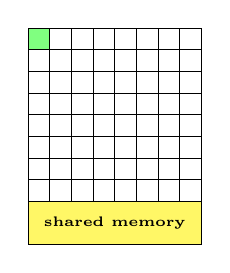
\begin{tikzpicture}[x=0mm, y=0mm, node distance=0 mm,outer sep = 0pt]
\tikzstyle{core}=[
    draw,
    rectangle,
    minimum height=\gpucoreheight,
    minimum width=\gpucorewidth,
    fill=green!50,
    anchor=north west]
\tikzstyle{coreidle}=[
    draw,
    rectangle,
    minimum height=\gpucoreheight,
    minimum width=\gpucorewidth,
    fill=white,
    anchor=north west]
\tikzstyle{shared}=[
    draw,
    rectangle,
    minimum height=\sharedheight,
    minimum width=\smxwidth,
    fill=yellow!60,
    anchor=north west]
\tikzstyle{gpucache}=[
    draw,
    rectangle,
    minimum height=\gpucacheheight,
    minimum width=\gpucachewidth,
    fill=blue!20,
    anchor=north west]
    \node[core] (core0) at(0mm,0mm) {};
\node[coreidle] (core1) [right = of core0] {};
\node[coreidle] (core2) [right = of core1] {};
\node[coreidle] (core3) [right = of core2] {};
\node[coreidle] (core4) [right = of core3] {};
\node[coreidle] (core5) [right = of core4] {};
\node[coreidle] (core6) [right = of core5] {};
\node[coreidle] (core7) [right = of core6] {};


\node[coreidle] (core8) [below = of core0] {};
\node[coreidle] (core9) [right = of core8] {};
\node[coreidle] (core10) [right = of core9] {};
\node[coreidle] (core11) [right = of core10] {};
\node[coreidle] (core12) [right = of core11] {};
\node[coreidle] (core13) [right = of core12] {};
\node[coreidle] (core14) [right = of core13] {};
\node[coreidle] (core15) [right = of core14] {};


\node[coreidle] (core16) [below = of core8] {};
\node[coreidle] (core17) [right = of core16] {};
\node[coreidle] (core18) [right = of core17] {};
\node[coreidle] (core19) [right = of core18] {};
\node[coreidle] (core20) [right = of core19] {};
\node[coreidle] (core21) [right = of core20] {};
\node[coreidle] (core22) [right = of core21] {};
\node[coreidle] (core23) [right = of core22] {};


\node[coreidle] (core24) [below = of core16] {};
\node[coreidle] (core25) [right = of core24] {};
\node[coreidle] (core26) [right = of core25] {};
\node[coreidle] (core27) [right = of core26] {};
\node[coreidle] (core28) [right = of core27] {};
\node[coreidle] (core29) [right = of core28] {};
\node[coreidle] (core30) [right = of core29] {};
\node[coreidle] (core31) [right = of core30] {};


\node[coreidle] (core32) [below = of core24] {};
\node[coreidle] (core33) [right = of core32] {};
\node[coreidle] (core34) [right = of core33] {};
\node[coreidle] (core35) [right = of core34] {};
\node[coreidle] (core36) [right = of core35] {};
\node[coreidle] (core37) [right = of core36] {};
\node[coreidle] (core38) [right = of core37] {};
\node[coreidle] (core39) [right = of core38] {};


\node[coreidle] (core40) [below = of core32] {};
\node[coreidle] (core41) [right = of core40] {};
\node[coreidle] (core42) [right = of core41] {};
\node[coreidle] (core43) [right = of core42] {};
\node[coreidle] (core44) [right = of core43] {};
\node[coreidle] (core45) [right = of core44] {};
\node[coreidle] (core46) [right = of core45] {};
\node[coreidle] (core47) [right = of core46] {};


\node[coreidle] (core48) [below = of core40] {};
\node[coreidle] (core49) [right = of core48] {};
\node[coreidle] (core50) [right = of core49] {};
\node[coreidle] (core51) [right = of core50] {};
\node[coreidle] (core52) [right = of core51] {};
\node[coreidle] (core53) [right = of core52] {};
\node[coreidle] (core54) [right = of core53] {};
\node[coreidle] (core55) [right = of core54] {};


\node[coreidle] (core56) [below = of core48] {};
\node[coreidle] (core57) [right = of core56] {};
\node[coreidle] (core58) [right = of core57] {};
\node[coreidle] (core59) [right = of core58] {};
\node[coreidle] (core60) [right = of core59] {};
\node[coreidle] (core61) [right = of core60] {};
\node[coreidle] (core62) [right = of core61] {};
\node[coreidle] (core63) [right = of core62] {};
\node[shared] (memory) at(0mm,-22.0mm) {\bfseries \tiny shared memory};


\end{tikzpicture}

\end{document}


